% ****** Start of file apssamp.tex ******
%
%   This file is part of the APS files in the REVTeX 4.1 distribution.
%   Version 4.1r of REVTeX, August 2010
%
%   Copyright (c) 2009, 2010 The American Physical Society.
%
%   See the REVTeX 4 README file for restrictions and more information.
%
% TeX'ing this file requires that you have AMS-LaTeX 2.0 installed
% as well as the rest of the prerequisites for REVTeX 4.1
%
% See the REVTeX 4 README file
% It also requires running BibTeX. The commands are as follows:
%
%  1)  latex apssamp.tex
%  2)  bibtex apssamp
%  3)  latex apssamp.tex
%  4)  latex apssamp.tex
%
\documentclass[%
%%%%%ok reprint,
%superscriptaddress,
%groupedaddress,
%unsortedaddress,
%runinaddress,
%frontmatterverbose, 
preprint,
%showpacs,preprintnumbers,
nofootinbib,
%nobibnotes,
%bibnotes,
 amsmath,amssymb,
 aps,
%pra,
%prb,
%rmp,
%prstab,
%prstper,
floatfix,
]{revtex4-1}

\usepackage{graphicx}% Include figure files
\usepackage{setspace}
\usepackage{dcolumn}% Align table columns on decimal point
\usepackage{bm}% bold math
%\usepackage[caption=false]{subfig}% bold math
\usepackage{subcaption}% bold math
%\usepackage{hyperref}% add hypertext capabilities
%\usepackage[mathlines]{lineno}% Enable numbering of text and display math
%\linenumbers\relax % Commence numbering lines

%\usepackage[showframe,%Uncomment any one of the following lines to test 
%%scale=0.7, marginratio={1:1, 2:3}, ignoreall,% default settings
%%text={7in,10in},centering,
%%margin=1.5in,
%%total={6.5in,8.75in}, top=1.2in, left=0.9in, includefoot,
%%height=10in,a5paper,hmargin={3cm,0.8in},
%]{geometry}

\begin{document}

\preprint{draft}

\title{ 
Transition Radiation Detector for the GlueX experiment
}% Force line breaks with \\
%\thanks{Thanks to everybody who contributed to this work}%
\author{Sergey Furletov}
\author{Lubomir Pentchev}
\affiliation{Thomas Jefferson National Accelerator Facility, Newport News, Virginia 23606, USA}
%
%\author{Ann Author}
% \altaffiliation[Also at ]{Physics Department, XYZ University.}%Lines break automatically or can be forced with \\
%\author{Second Author}%
% \email{Second.Author@institution.edu}
%\affiliation{%
% Authors' institution and/or address\\
% This line break forced with \textbackslash\textbackslash
%}%

%\collaboration{GlueX Collaboration}%\noaffiliation


\date{\today}% It is always \today, today,
             %  but any date may be explicitly specified

\begin{abstract}
We propose to build a Transition Radiation Detector (TRD) 
with Gaseous Electron Multiplier (GEM) amplification, referred as GEM-TRD,
to improve the electron-pion separation in the GlueX experiment.
It will allow to study precisely reactions with 
electron-positron pairs in the final states; such reactions like
$J/\psi $ photoproduction near threshold have significant impact
in many fields of the particle physics.
The motivation for such an upgrade is followed by a 
technical description of the detector and the electronics. 
Preliminary requirements for the GEM-TRD gas system are specified. 
\end{abstract}

%\pacs{Valid PACS appear here}% PACS, the Physics and Astronomy
%                             % Classification Scheme.
%%\keywords{Suggested keywords}%Use showkeys class option if keyword
%                              %display desired
\maketitle

%\tableofcontents

\clearpage
\mbox{~}
%\section{Formulation of the problem}

\section{Motivation}

Important features of the GlueX detector include full acceptance,
charge and neutral particle registration, and high-rate
electronics and DAQ, however it has limited PID capabilities.
A DIRC detector was built for the phase-II of the GlueX experiment 
and used for pion/kaon separation that will extend the GlueX program
by including strangeness physics.
Another important extension of the program 
would be the di-electron physics.
The GlueX detector has the unique possibility to study the $J/\psi $
photoproduction off the proton near threshold in the full kinematic space. 
As the $J/\psi $-proton interaction is mediated predominantly by gluons,
such studies allow to probe the gluonic content of the proton:
mass radius, anomalous contribution to the mass of the proton, 
the gluonic GPD; all these properties are not accessible with
electro-magnetic probes.
First results of the $J/\psi $ photoproduction near threshold \cite{prl_gluex},
published by GlueX in 2019, collected already 100+ citations. 
Such studies, however, are limited by the huge pion background
that can mimic the electron-positron pairs used to identify 
the $J/\psi $ particle. 
The suppression of the pion background would allow to study
the Bethe-Heitler process that has the same $e^+e^-p$ particles
in the final state.
As an electro-magnetic process it is fully calculable and would
allow to reduce the systematics of the $J/\psi $ photoproduction
significantly.

The pions are about four orders of magnitude more numerous 
than the electrons.
The electro-magnetic calorimeters reduce the background pion
pairs by a similar magnitude, when selections are applied to both, 
the electron and the positron candidates. 
In this case statistical analysis are needed to estimate 
the electron-positron yields, with a signal-to-background ratio of about one,
resulting in significant systematic uncertainties.
Another factor of 10 suppression is needed to be able to study
reactions with $e^+e^-$ pairs in the final state on event-by-event basis.
This can be achieved with a Transition Radiation Detector (TRD)
consisting of a radiator, drift volume filled with Xe gas mixture,
and an amplification stage employing Gaseous Electron Multiplier 
(GEM) technology \cite{NIM_GEM_TRD}. 
Such GEM-TRD detector will serve not only as a particle-identification 
device, but also as a tracker with a potential to improve 
the momentum resolution and the precision of the tracks extrapolated to
the DIRC detector.

\section{The GEM-TRD detector}

The proposed detector will be placed in the forward region
of the GlueX detector just at the downstream face of the solenoid,
see Figs. \ref{fig:side_view},\ref{fig:front_view}.
It will consists of two separate chambers,
each providing $1392 \times 528$~mm$^2$ sensitive area. 
The frames of the chambers holding the front-end electronics
will be outside of the acceptance (Fig. \ref{fig:front_view}).
\begin{figure}[]
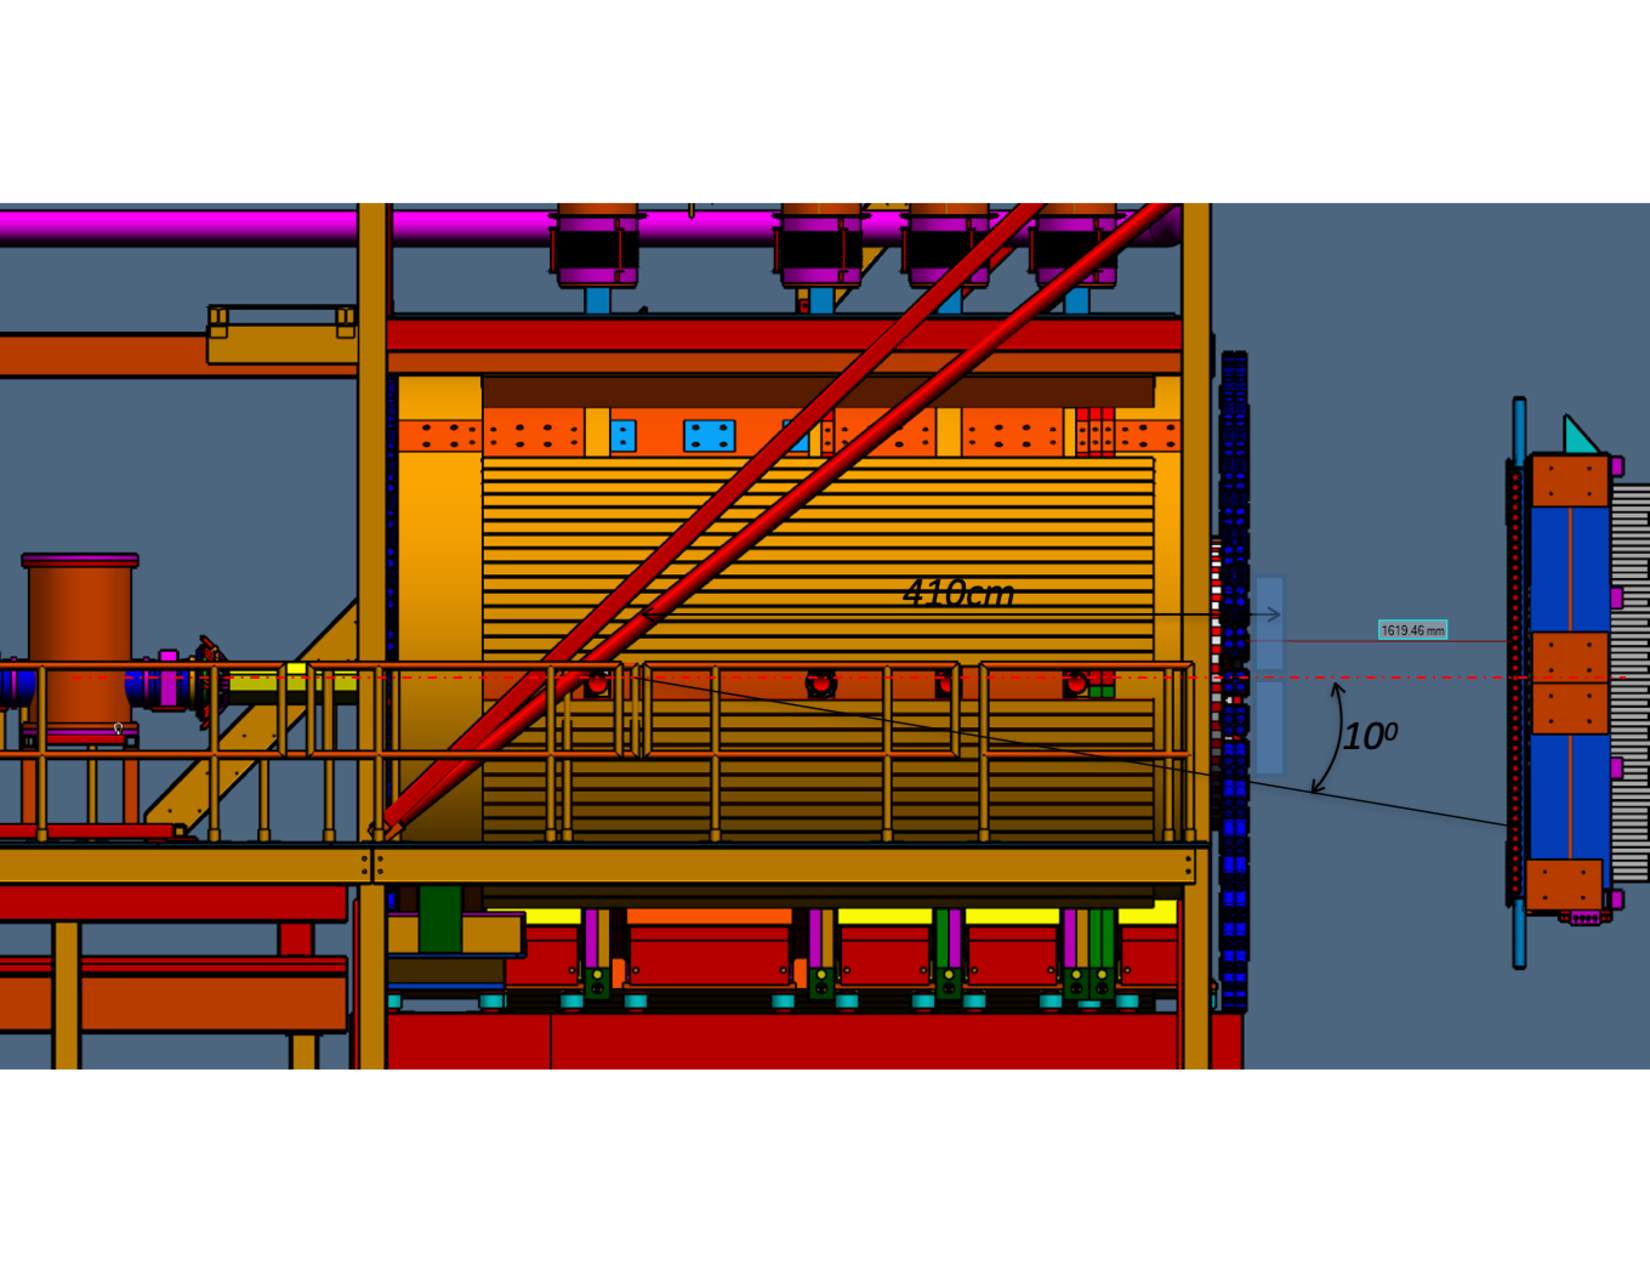
\includegraphics[width=0.80\textwidth]{./fig/GEM_TRD_side.pdf}
  \caption{
Side view showing the approximate position of the proposed GEM-TRD detector
(light blue boxes), at $410$~cm downstream of the target,
covering $86$\% of the forward GlueX acceptance of $\sim 10^\circ$ 
polar angle.
}
  \label{fig:side_view}
\end{figure}
\begin{figure}[]
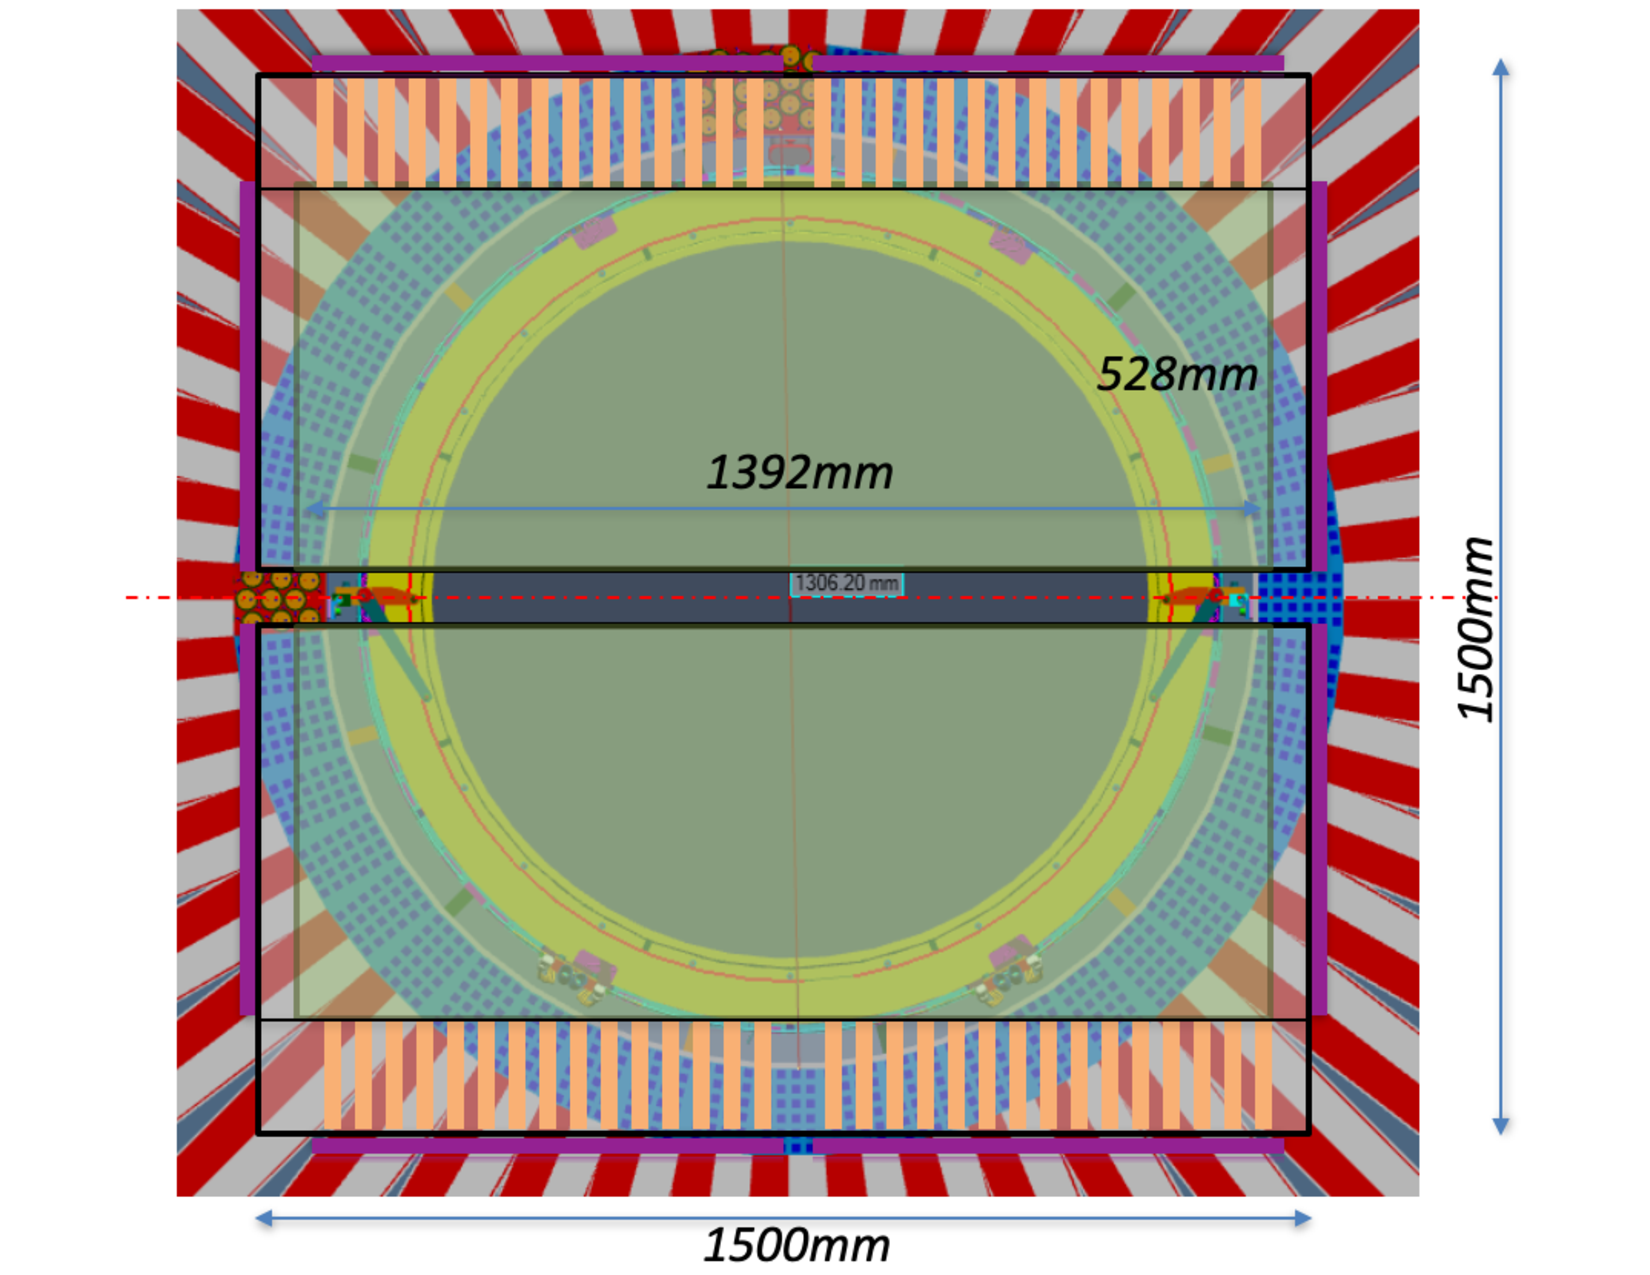
\includegraphics[width=0.80\textwidth]{./fig/GEM_TRD_full.pdf}
  \caption{
Front view of the GEM-TRD detector placed at the face of the solenoid
magnet. It consists of two separate chambers with $1392 \times 528$~mm$^2$
sensitive area. All the frames holding the front-end electronics
(purple thick lines) 
of sizes $\sim 1500 \times 1500$~mm$^2$
are outside of the GlueX forward acceptance.
}
  \label{fig:front_view}
\end{figure}

The detector has a radiator layer $15$~cm thick, followed 
by a $2$~cm drift volume, and a GEM stage combined with a readout board.
The principle of operation is illustrated in Fig.\ref{fig:principle}.
The Transition Radiation (TR) photons in the $keV$ region produced by the 
electrons in the radiator are absorbed by the Xe gas mixture in the drift volume
emitting electrons that drift to and are amplified by the GEM. 
The signals are readout from  X- and Y-strips on the readout board.
The horizontal strips are separated in the middle and readout 
from the left and right side of the chambers (Fig. \ref{fig:front_view}).
The strip pitch is $1$~mm, resulting in $2,448$ electronic channels
per chamber, or $4,896$ in total.
The signals are amplified on-board and then digitized with flash ADCs
using the same electronics as for the GlueX drift chambers: GASII \cite{GASII}
preamps and flashADC-125 \cite{fADC125}.
Thus we record the energy deposition along the track 
(measured by the drift time)
that has different profile for the TR photons
absorbed predominately at the entrance, and the track ionization 
that has uniform distribution, see Fig.\ref{fig:profile}. 
At the same time such detector works as a Time Projection Chamber,
allowing to reconstruct the track segment within the drift volume.

\begin{figure}[h]
  \begin{subfigure}[b]{0.40\textwidth}
    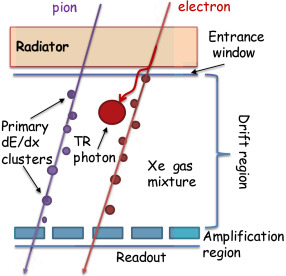
\includegraphics[width=\textwidth]{./fig/GEM_TRD_principle.jpg}
    \caption{GEM-TRD principle}
    \label{fig:principle}
  \end{subfigure}
  %
  \begin{subfigure}[b]{0.49\textwidth}
    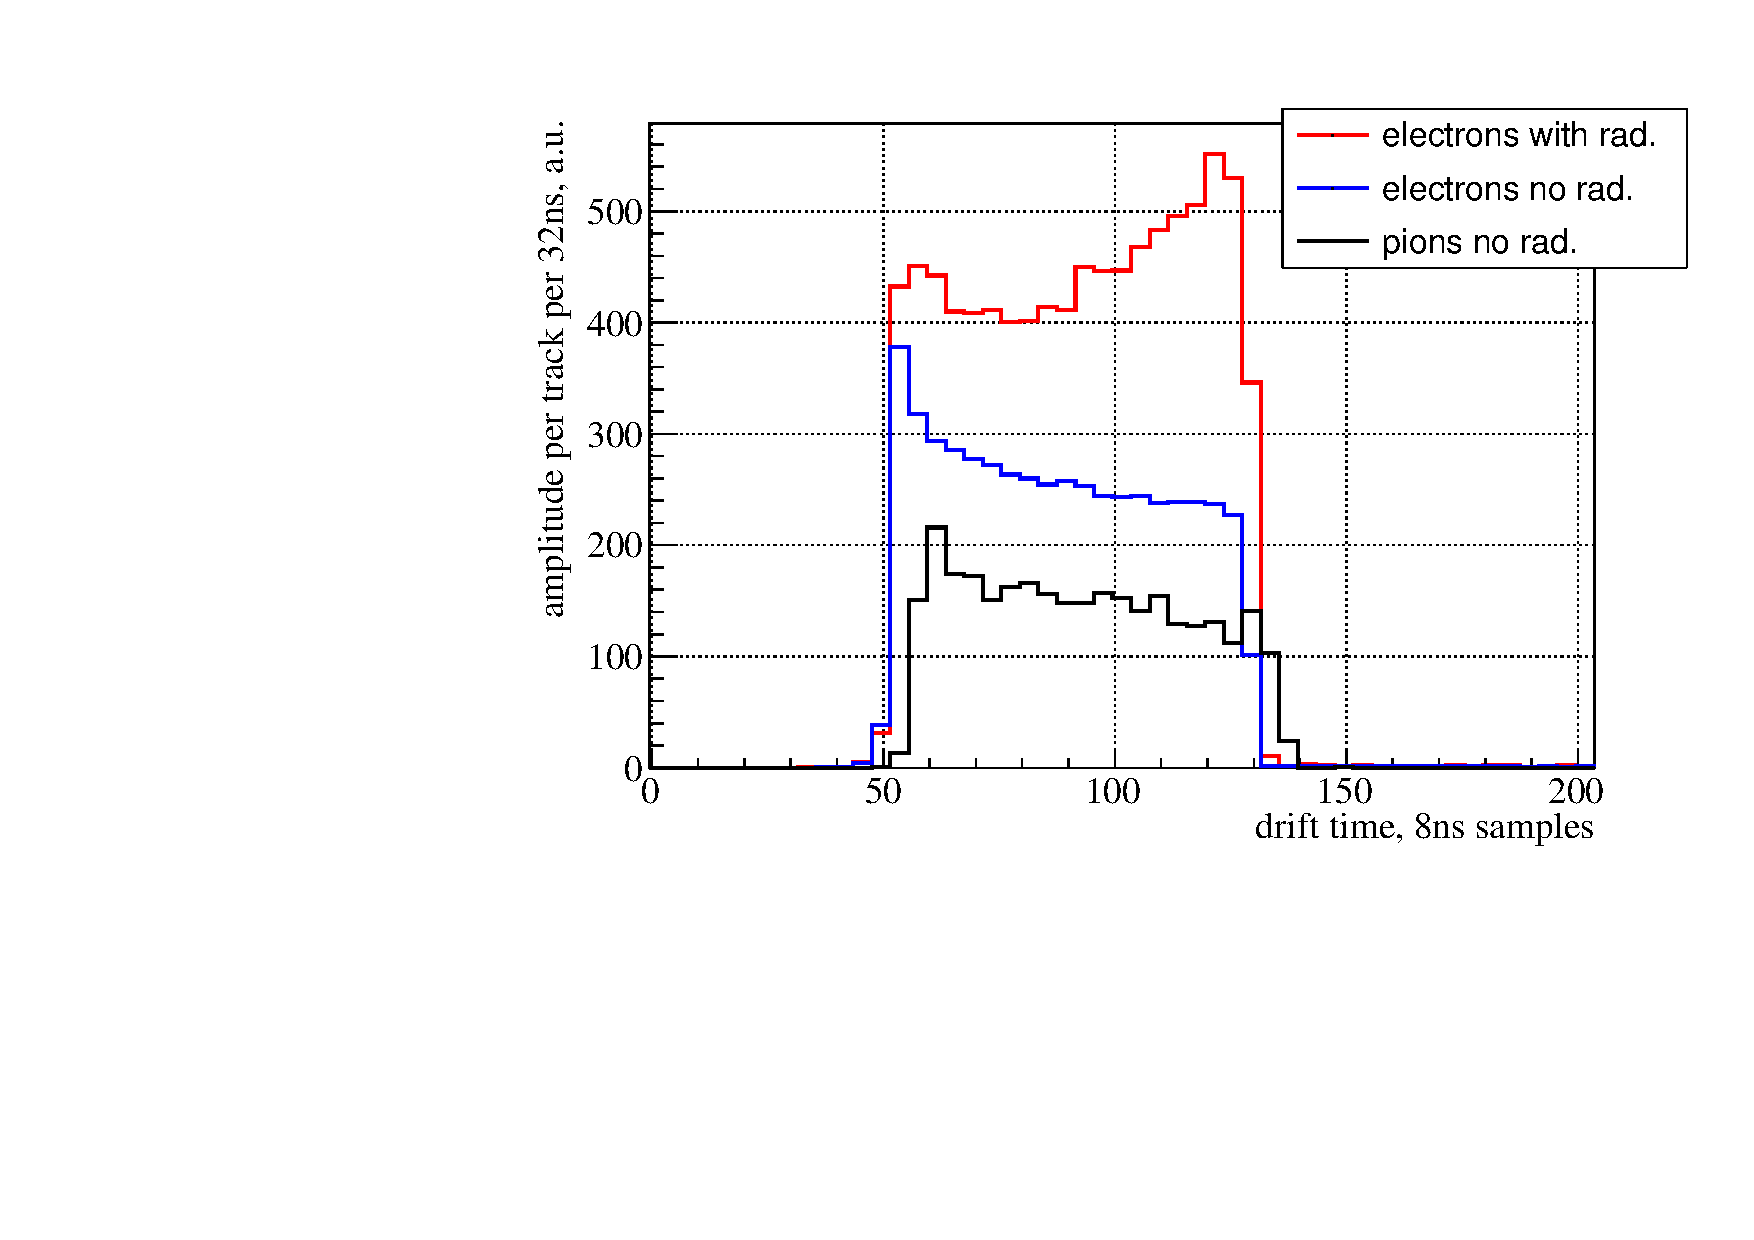
\includegraphics[width=\textwidth]{./fig/GEMTRD_piel_ampl_vs_t_left-2142.pdf}
    \caption{Amplitude profiles for electrons with and without radiator and pions;
data from studies with small prototypes}
    \label{fig:profile}
  \end{subfigure}
  \caption{
}
  \label{fig:BH_pove_pi}
\end{figure}

\begin{figure}[]
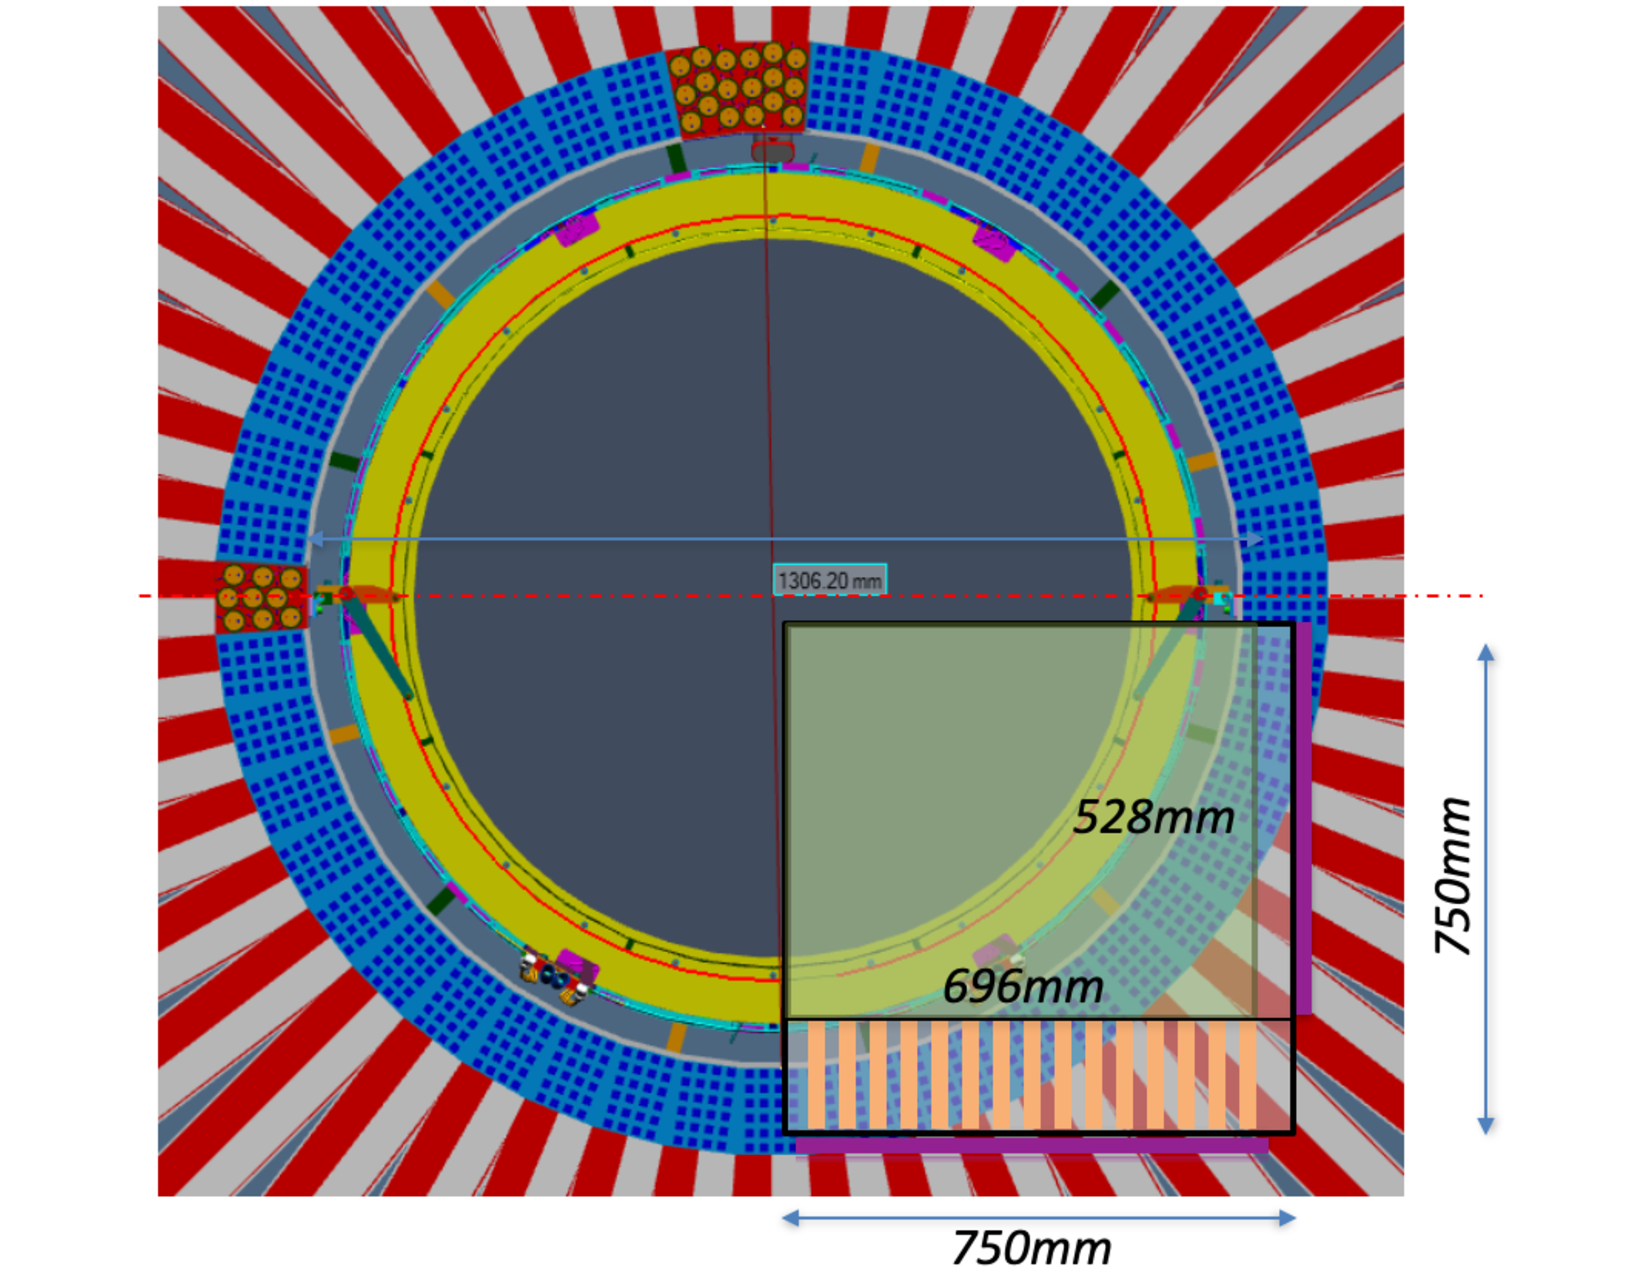
\includegraphics[width=0.80\textwidth]{./fig/GEM_TRD_prototype.pdf}
  \caption{
Front view of the GEM-TRD large-scale prototype
that has $696 \times 528$~mm$^2$ 
sensitive area. 
}
  \label{fig:proto}
\end{figure}

\begin{table}[hp]
\begin{ruledtabular}
\begin{tabular}{lcc}
\textrm{parameter}&
\textrm{value}&
\textrm{comment}\\
\colrule
sensitive area & $2 \times (1392 \times 528$~mm$^2)$ & two separate chambers\\
frame-free area & $1500 \times 1500~$mm$^2$ & except some minimal support \\
distance from the target & $4100$~mm & \\
forward acceptance coverage & $86$\% & for $e^+e^-$ invariant mass $>1.2$~GeV \\
radiator thickness & $150$~mm & \\
drift volume thickness & $20$~mm & \\
total detector thickness & $<4$\% R.L. & \\
drift field & $1.5$~kV/cm & \\
gas mixture & Xe/CO$_2$ $90/10$ & \\
maximum drift time & $800$~ns & \\
gas amplification & $\sim 5.10^4$ & \\
strip types & X and Y & on the same layer with capacitive coupling \\
strip pitch & $1$~mm & \\
readout channels & $4,896$ & $2,448$ per chamber \\
GASII pre-amps (24 channels) & $204$ & $102$ per chamber \\
GASII amplification & $2.4$ mV/fC & \\
flashADC-125 (72 channels) & $68$ & $34$ per chamber \\ 
VXS crates & 5 & \\
\end{tabular}
\end{ruledtabular}
\caption{
Main parameters of the GEM-TRD detector.
\label{tab:tech}
}
\end{table}
The main parameters of the GEM-TRD detector are given in Table \ref{tab:tech}.
They are based on tests with small prototypes ($10\times10$~cm$^2$)
done during the past several years, as discussed in the next section,
and are preliminary.
Further optimization of the detector will be done with a large-scale prototype
that will be built and tested during the 2022 and 2023 running periods.
This prototype will cover a quarter of the final detector (Fig.\ref{fig:proto}),
allowing to be used for real physics data taking.
The electronics of the prototype will be re-used in the final detector.


\section{Studies with small-scale prototypes}
 
\begin{figure}[h]
  \begin{subfigure}[b]{0.49\textwidth}
    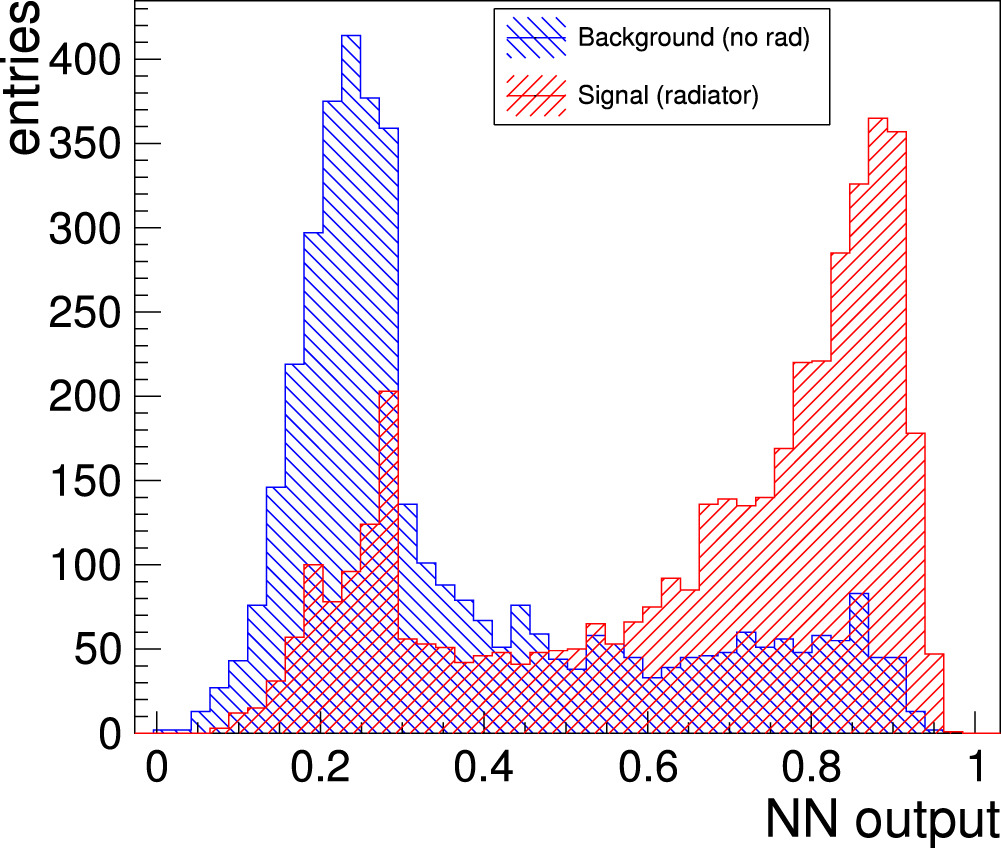
\includegraphics[width=\textwidth]{./fig/GEM_TRD_NNoutput.jpg}
    \caption{Neural Network (NN) output for electrons with and without 
radiator}
    \label{fig:NNout}
  \end{subfigure}
  %
  \begin{subfigure}[b]{0.40\textwidth}
    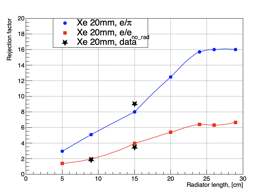
\includegraphics[width=\textwidth]{./fig/pion_rejection.png}
    \caption{Pion rejection factor from data (stars) 
and simulations from radiator/no radiator (red)
and electron/pion (blue) comparison;
data from studies with small prototypes}
    \label{fig:profile}
  \end{subfigure}
  \caption{
}
  \label{fig:BH_pove_pi}
\end{figure}




\newpage
\section{Gas System Requirements}
The high price of the Xe gas requires system that recirculates
and purifies the gas mixture.
Each GEM-TRD module has two gas volumes - 
the main one filled with $Xe/CO_2$ gas mixture of $90/10\%$ 
containing the drift and the amplification volumes,
and the second one for the radiator filled with CO2. 
The thickness of the drift and amplification volume is $20$~mm and $10$~mm respectively.
Thus, we estimate the $Xe/CO_2$ gas volume to be $25$~l per chamber, or $50$~l in total.
For the $CO_2$ volume it has a thickness of $150$~mm or $125$~l per module and $250$~l total.
For the $Xe/CO_2$ volume we aim to have 8 volume exchanges per day, i.e. $20$~l/h.
The $CO_2$ volume can be exchanged once  per day or $5$~l/h.

The entrance and exit gas windows will be made of $100$~$\mu$m Mylar, possibly enforced with Rochacell
material.
The detector will allow operation with overpressure between $0.5$ and $2$~mbar.
The two gas volumes will be separated by $50$~$\mu$m Mylar, covered with $1$~$\mu$m $Al$.
To limit the variations of the drift field, we require the pressure difference between the two gas
volumes to be less than $0.2$~mbar. 

Oxygen contamination and water vapor should be kept less than $50$~ppm, 
to minimize the electron recombination 
in the drift volume. The Nitrogen contamination should be kept less than $0.5\%$.

The elements of the gas system that operate above $1$~bar should be kept in a separate gas room,
elevated approximately $7$~m above the detector. They will be connected to the detector with
gas lines of about $50$~m length.

The parameters and requirements of the gas system are summarized in Table \ref{tab:gas}.

\begin{table}[hp]
\begin{ruledtabular}
\begin{tabular}{lcc}
\textrm{item}&
\textrm{requirement}&
\textrm{comment}\\
\colrule
total $Xe/CO_2$  gas volume & $50$ l &\\
total $CO_2$ gas volume & $250$ l &\\
$Xe/CO_2$  gas flow & $20$ l/h &\\
$CO_2$ gas flow & $5$ l/h &\\
Operating overpressure & $0.5-2$~mbar &\\
Pressure difference b/n two volumes & $<0.2$~mbar &\\
Oxygen contamination & $<50$~ppm &\\
water vapor & $<50$~ppm &\\
Nitrogen contamination & $<0.5\%$ &\\
\end{tabular}
\end{ruledtabular}
\caption{
General parameters and requirements for the GlueX TRD gas system.
\label{tab:gas}
}
\end{table}


\bibliography{gem_trd.bib}% Produces the bibliography via BibTeX.

\end{document}
%
% ****** End of file apssamp.tex ******
